\chapter{Основні поняття криптології. Теорія секретних систем Шеннона}

У першій лекції ми познайомились з деякими початковими поняттями криптології. Як
там відмічено, до роботи Клода Шеннона ,,Теорія зв'язку в
секретних системах'', що вийшла з друку в 1949 році, криптографія складалася з 
окремих шифрів, інколи досить стійких на той час, та деяких правил злому
шифрів. Успіх в криптоаналітичних атаках та створенні надійних засобів
шифрування  залежав від винахідливості, уміння, майстерності їх авторів, тобто
був суто індивідуальним і погано передбачуваним. Шеннон на основі розробленої
ним раніше (під впливом актуальних задач криптографії і зв’язку) математичної
теорії інформації запропонував формальні моделі криптографічних систем, дав
математичні визначення базових понять криптографії. Тепер задачі і проблеми
криптографії можна було розглядати в математичних термінах, застосовувати
математичні методи аналізу та доведення. У подальшому теоретична криптографія 
перетворилася в прикладну математичну дисципліну, що і зараз знаходиться  у
процесі інтенсивного розвитку та розробки нових методів і понять, уточнення
раніше введених, формулюванні нових цілей та задач. 

\section{Основні поняття криптології}
{\centering\itshape (див. також лекцію \ref{lecture:1}) \par}

\begin{definition}[Відкритий текст(ВТ)]
    Відкритий текст(ВТ) --- повідомлення, дані, елемент простору повідомлень,
    до якого застосовується процедура криптографічного перетворення, шифрування.
    Звичайно, під ВТ розуміють текст, заданий у вигляді послідовності символів
    скінченого алфавіту, з доступним семантичним змістом. ВТ
    отримують після вірного розшифрування.
\end{definition}

\begin{definition}[Шифрований текст, шифротекст  або криптограма (ШТ)]
    Шифрований текст, шифротекст  або криптограма (ШТ) --- інформація, яка
    отримана в після застосування до відкритого тексту процедури зашифрування.
\end{definition}

\begin{definition}[Зашифрування]
    Зашифрування --- криптографічне перетворення повідомлення, ВТ з
    застосуванням таємних ключів, в результаті якого буде отримано шифротекст
    або криптограму (ШТ) з недоступним для незаконного користувача семантичним
    змістом.
\end{definition}

\begin{definition}[Розшифрування]
    Розшифрування --- зворотне криптографічне перетворення ШТ з застосуванням
    таємних ключів, в результаті цієї процедури законний користувач отримує ВТ,
    що був зашифрований.  Використовують для даної процедури також термін
    дешифрування.
\end{definition}

\begin{definition}[Шифратор]
    Шифратор --- пристрій, що здійснює процедуру зашифрування.
\end{definition}

\begin{definition}[Дешифратор]
    Дешифратор --- пристрій, що виконує процедуру розшифрування.
\end{definition}

\begin{definition}[Криптографічна система]
    Криптографічна система --- система забезпечення безпеки інформації
    криптографічними методами, перш за все у конфіденційності, цілісності,
    автентичності, доступності. З практичної точки зору -  це набір апаратних і
    (або) програмних засобів, інструкцій і правил, за допомогою яких,
    використовуючи криптографічні перетворення, можна зашифрувати повідомлення і
    розшифрувати криптограму різними способами, один із яких вибирається за
    допомогою секретного ключа, а також здійснювати інші криптографічні
    протоколи. Математичну модель Шеннона криптографічної системи буде
    розглянуто у цій лекції.
\end{definition}

\begin{definition}[Криптографічна стійкість]
    Криптографічна стійкість --- у широкому розумінні --- це здатність
    криптосистеми або криптоалгоритму протистояти атакам з використанням методів
    криптоаналізу; у вузькому розумінні (практична стійкість) --- чисельна
    характеристика часової та місткісної складності розкриття криптографічного
    алгоритму з урахуванням тих науково-технічних методів та засобів, які може
    використати криптоаналітик.
\end{definition}

\begin{definition}[Теоретична стійкість]
    Теоретична стійкість ---  у широкому розумінні --- це стійкість
    криптосистеми за наявності у криптоаналітика необмеженого часу, необмежених
    обчислювальних ресурсів, якнайкращих методів криптоаналізу, у вузькому
    розумінні --- це в деякому сенсі гарантована стійкість. Основні підходи до
    визначення поняття теоретичної стійкості нині розглядаються у рамках деяких
    математичних моделей. Так, розглядається стійкість теоретико-інформаційна,
    теоретико-складнісна, довідна.
\end{definition}

\begin{definition}[Практична стійкість]
    Практична стійкість --- стійкість криптосистеми на теперішній час з
    урахуванням того, що криптоаналітик володіє обмеженим часом,
    обмеженими обчислювальними ресурсами і сучасними методами криптоаналізу,  а
    також чисельна характеристика часової та місткісної складності розкриття
    криптографічного алгоритму.
\end{definition}

\section{Основні види криптографічних атак (нападів) залежно від типу відомої
    інформації}

В криптології загально прийняте наступне правило: 
\begin{definition}[Правило Керкгоффа]
    стійкість криптосистеми не повинна спиратися на секретність її будови,
    алгоритму шифрування, а повинна ґрунтуватися на секретності ключа (при
    надійному алгоритмі шифрування і достатньому розмірі ключа). 
\end{definition}

Згідно з додатковою інформацією атаки класифікуються у порядку їх посилення
наступним чином:
\begin{enumerate}
    \item\label{item:attack:CT} \textit{Атака на основі ( з використовуванням) тільки шифротекста}. У криптоаналітика є шифротексти декількох повідомлень,
        зашифрованих одним і тим самим алгоритмом шифрування і невідомим ключем
        (ключами). Задача криптоаналітика полягає в розкритті відкритого тексту
        як можна більшого числа повідомлень або, що краще, отриманні ключа
        (ключів), використаних для шифрування повідомлень з метою дешифрування
        також і інших повідомлень, зашифрованих тими ж ключами.
\item\label{item:attack:OT} \textit{Атака на основі (з використанням)
    відкритого тексту}. У криптоаналітика є доступ не тільки до шифротекстів
    декількох повідомлень, але і до відповідних відкритих текстів цих
    повідомлень. Його задача полягає в отриманні ключа (або ключів),
    використаного (використаних) для шифрування повідомлень з метою
    дешифрування інших повідомлень, зашифрованих тим же ключем (ключами).
\item\label{item:attack:chosenOT} \textit{Атака на основі вибраного відкритого
    тексту.} У криптоаналітика не тільки є доступ до шифротекстів і відповідних
    відкритих текстів декількох повідомлень, але є й можливість вибирати
    відкритий текст (тексти) і отримати шифрований (шифровані). Це надає більше
    варіантів, ніж атака з використанням відкритого тексту, оскільки
    криптоаналітик буде вибирати  відкриті тексти зі спеціальними
    властивостями, що може надати більше інформації про ключ. Його задача
    полягає в отриманні ключа (або ключів), використаного для шифрування
    повідомлень, або алгоритму, що дозволяє дешифрувати нові повідомлення,
    зашифровані тим  же ключем (або ключами).
\item\label{item:attack:adaptiveOT} \textit{Адаптивна атака з використанням
    відкритого тексту.} Криптоаналітик не тільки може вибирати тексти для
    шифрування, але також може будувати свій подальший вибір текстів на базі
    одержаних результатів шифрування попередніх .  При розкритті з
    використанням вибраного відкритого тексту криптоаналітик міг вибрати для
    шифрування тільки один або декілька ВТ одночасно для отримання відповідних
    ШТ, при адаптивному нападі з використанням вибраного відкритого тексту він
    може вибрати спочатку один ВТ і отримати криптограму, потім вибрати
    наступний ВТ, використовуючи результати першого вибору та шифрування, і так
    далі. Атаки \ref{item:attack:OT}, \ref{item:attack:chosenOT},
    \ref{item:attack:adaptiveOT} можливі, наприклад, при шифруванні з відкритим
    ключем.  \item\label{item:attack:chosenCT} \textit{Атака на основі
    вибраного шифротекста.} Криптоаналітик може вибрати різні шифротексти для
    розшифрування і має доступ до розшифрованих відкритих текстів (наприклад,
    криптоаналітик має доступ до апарату-шифратора).
\item\label{item:attack:adaptiveChosenCT} \textit{Адаптивна атака на основі
    вибраного шифротекста.} Криптоаналітик має можливість для ШТ, що послідовно
    вибираються з урахуванням попередніх результатів, отримувати відповідні ВТ
    (аналогічно п. \ref{item:attack:adaptiveOT}). Задача знайти таємний ключ,
    або дешифрувати інші повідомлення. Атаки п. \ref{item:attack:chosenOT},
    \ref{item:attack:adaptiveChosenCT} особливо небезпечні для криптосистем з
    відкритим ключем.  \item Атака на основі вибраного тексту  --- об'єднує
    можливості атак п. \ref{item:attack:chosenOT}, п.
    \ref{item:attack:chosenCT}.  \item Адаптивна атака на основі вибраного
    тексту  --- об'єднує можливості атак п. \ref{item:attack:adaptiveOT},
    п. \ref{item:attack:adaptiveChosenCT}.
\end{enumerate}

Атаки в цьому списку з більшим номером загалом сильніші і небезпечніші ніж з
меншим. Для всіх сучасних шифраторів обов'язкова вимога --- стійкість до атаках
типу 1 і 2. Якщо у криптоаналітика є деяка додаткова інформація про ключі
(окрім їх довжини) або про зв'язок між різними ключами, то напади на
криптосистему  стають ще небезпечнішими. До такої атаки належить, зокрема, атака
з використанням інформації з так званого побічного каналу, що міститься,
наприклад, в електромагнітному випромінюванні шифратора.

\section{Загальна схема секретного зв'язку. Математична модель криптосистеми}

Розглянемо загальну схему криптографічного захисту зв’язку за допомогою
симетричних криптосистем.  Будемо позначати: $A$ --- відправник,
$B$ --- одержувач, $M$--- відкритий текст (ВТ); $C$ --- криптограма (ШТ)
відправника; $C'$ --- отримана криптограма ($C$ може бути змінена при передачі,
наприклад, через перешкоди). Ключ $k$ заздалегідь передається по закритому
каналу одержувачу (або і відправнику, і одержувачу із джерела ключів), при
цьому неможливо отримати незаконному користувачу ніякої інформації щодо ключа,
здійснити будь-яку зміну в ключі  (вважається, що канал цілком надійний).
Призначення рандомізатора --- використовуючи  зовнішнє джерело випадковості
попередньо зрівняти деякі частотні характеристики ВТ.  Криптоаналітик завжди
може зчитувати ШТ з каналу передачі, але не може змінювати криптограми або мати
якийсь вплив на передачу ( так званий пасивний криптоаналітик).

\begin{figure}
    \centering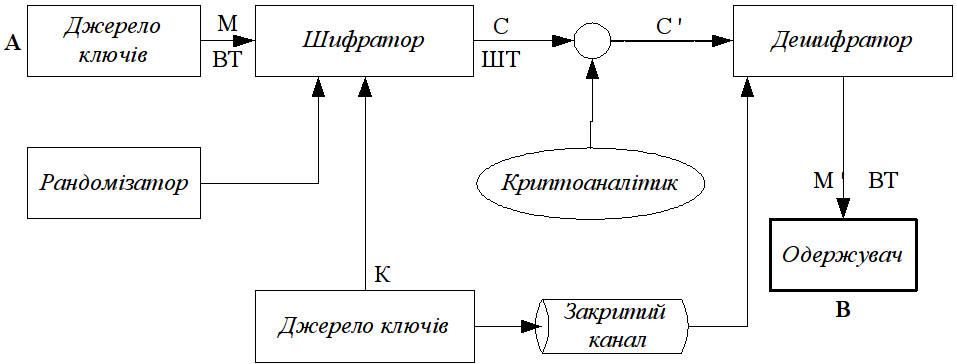
\includegraphics[width=5.0in]{crypt-img/crypt-img4.png}
    \caption{Загальна схема секретного зв'язку}\label{img:secretConnection}
\end{figure}
